\chapter{Neural Style Transfer}
\begin{styletransfer}
    Style transfer is the technique of recomposing images in the style of other images or we can say style transfer relies on separating the content and style of an image. Given one content image and one style image, we aim to create a new, target image which should contain our desired content and style components:
        \begin{itemize}
            \item objects and their arrangement are similar to that of the content image (feature reconstruction) 
            \item style, colors, and textures are similar to that of the style image (texture synthesis)
        \end{itemize}
     
\section{Content representation and loss}
    We can construct images whose feature maps at a chosen convolution layer match the corresponding feature maps of a given content image. We expect the two images to contain the same content, but not necessarily the same texture and style. Given a chosen content layer \textbf{l}, the content loss is defined as the Mean Squared Error between the feature map \textbf{F} of our content image \textbf{C} and the feature map \textbf{P} of our generated image \textbf{Y}.
    \[Lcontent = \frac{1}{2}\sum_{i j}^{ } \left ( Fij - Pij \right )^{2}\]
    When this content-loss is minimized, it means that the mixed-image has feature activation in the given layers that are very similar to the activation of the content-image. Depending on which layers we select, this should transfer the contours from the content-image to the mixed-image.

\section{Style representation and loss}

    We will do something similar for the style-layers, but now we want to measure which features in the style-layers activate simultaneously for the style-image, and then copy this activation-pattern to the mixed-image. One way of doing this, is to calculate the Gram-matrix(a matrix comprising of correlated features) for the tensors output by the style-layers. The Gram-matrix is essentially just a matrix of dot-products for the vectors of the feature activations of a style-layer.
    If an entry in the Gram-matrix has a value close to zero then it means the two features in the given layer do not activate simultaneously for the given style-image. And vice versa, if an entry in the Gram-matrix has a large value, then it means the two features do activate simultaneously for the given style-image. We will then try and create a mixed-image that replicates this activation pattern of the style-image.If the feature map is a matrix F, then each entry in the Gram matrix G can be given by:
    
   \[ Gij = \sum_{k}^{ } Fik Fjk \]

    The loss function for style is quite similar to out content loss, except that we calculate the Mean Squared Error for the Gram-matrices instead of the raw tensor-outputs from the layers.

    
   \[Lstyle = \frac{1}{2}  \left ( \sum_{i=0}^{L} \left ( Gij - Aij \right )^{2} \right )\]

    As with the content representation, if we had two images whose feature maps at a given layer produced the same Gram matrix we would expect both images to have the same style, but not necessarily the same content. Applying this to early layers in the network would capture some of the finer textures contained within the image whereas applying this to deeper layers would capture more higher-level elements of the image’s style. Gatys et. al [1] found that the best results were achieved by taking a combination of shallow and deep layers as the style representation for an image. The best results are achieved by a combination of many different layers from the network, which capture both the finer textures and the larger elements of the original image.
    \begin{figure}[h]
        \centering
        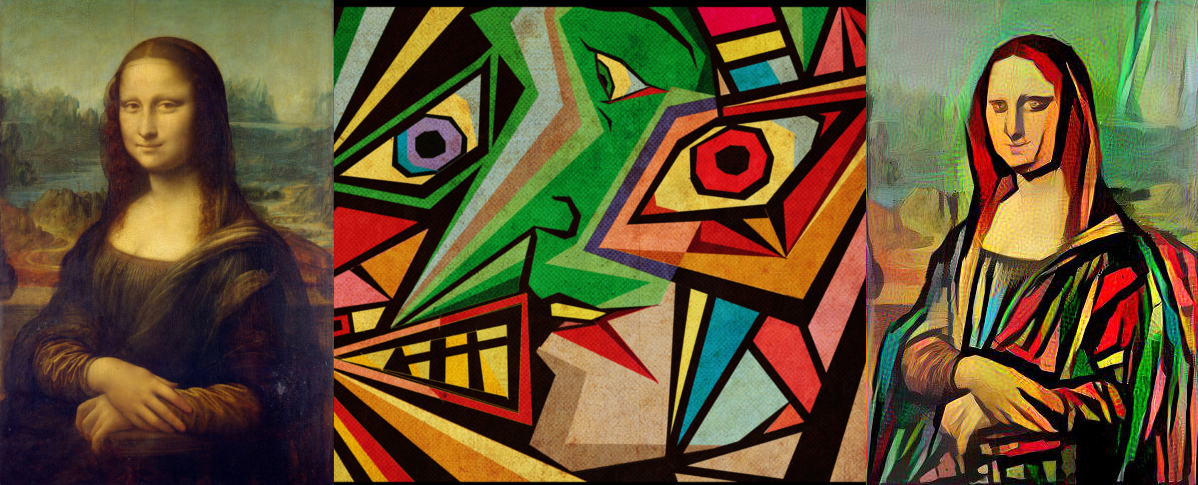
\includegraphics[width=0.8\linewidth]{styletransfer.png}
         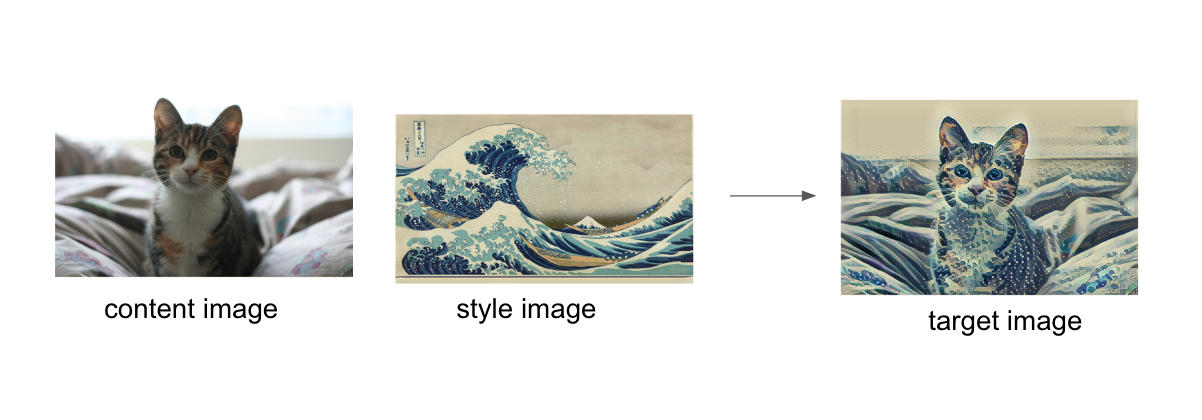
\includegraphics[width=0.8\linewidth]{styletransfercat.png}
        \caption{Style Transfer}
    \end{figure} 

\section{Optimizing loss function and styling the image}
    Using a pre-trained neural network such as VGG-16, an input image (i.e. an image which provides the content), a style image (a painting with strong style elements) and a random image (output image), one could minimize the losses in the network such that the style loss (loss between the output image style and style of ‘style image’), content loss (loss between the content image and the output image) and the total variation loss (which ensured pixel wise smoothness) were at a minimum. In such cases, the output image generated from such a network, resembled the input image and had the stylist attributes of the style image. The total loss can then be written as a weighted sum of the both the style and content losses. 
    \[Ltotal = \alpha Lcontent  + \beta Lstyle \]
    We will minimize our total loss by Adam optimizer. As our loss go down we will go close to our goal of producing a style transfer image Y.

\end{styletransfer}

